\documentclass[10pt,a4paper]{article}
\usepackage[UTF8]{ctex}
\usepackage[T1]{fontenc}
\usepackage{cite}
\usepackage{ctex}
\usepackage{amsmath,amsfonts,amssymb}
\usepackage{graphicx}% 图片插入宏包
\usepackage{subfigure}% 并排子图
\usepackage{setspace}
\setstretch{2}
\usepackage{float}% 浮动环境,用于调整图片位置
\usepackage[export]{adjustbox}% 防止过宽的图片
\usepackage{bibentry}
\usepackage{natbib}% 以上2个为参考文献宏包
\usepackage{abstract}% 两栏文档,一栏摘要及关键字宏包
\renewcommand{\abstracttextfont}{\fangsong}% 摘要内容字体为仿宋
\renewcommand{\abstractname}{\textbf{摘\quad 要}}% 更改摘要二字的样式
\usepackage{xcolor}% 字体颜色宏包
\usepackage{url}% 超链接
\usepackage{bm}% 加粗部分公式
\usepackage{multirow}
\usepackage{booktabs}
\usepackage{color}
\usepackage{epstopdf}
\usepackage{epsfig}
\usepackage{longtable}% 长表格
\usepackage{supertabular}% 跨页表格
\usepackage{algorithm}
\usepackage{algorithmic}
\usepackage{changepage}% 换页
\usepackage{enumerate}% 短编号
\usepackage{caption}% 设置标题
\usepackage{tabularx}
\usepackage{amsmath}

\usepackage[colorlinks=true, allcolors=blue]{hyperref}
\usepackage[left=2.50cm,right=2.50cm,top=2.80cm,bottom=2.50cm]{geometry}

\usepackage{fancyhdr} %设置全文页眉、页脚的格式




%------------------------------------------------------------

\title{液体表面张力系数测定}
\author{费维瀚 PB24000347 少年班学院}
\begin{document}
    \maketitle
    \begin{abstract}
       
    \end{abstract}

	\par \textbf{关键词}:表面张力系数,拉脱法,焦利氏秤,不确定度分析,曲线拟合
	\section*{引言}
    
	\section{实验原理}
    
    \section{仪器与方法}
    
    \section{数据与讨论}
        \subsection{锥形弹簧弹性系数}
        \subsubsection{实验数据}
            
        \subsection{自来水表面张力系数}
        \subsubsection{实验数据}

        \begin{table}[H]
            \centering
            \begin{tabular}{|c|c|c|c|c|c|c|}
                \hline
                \textbf{洗洁精浓度} & \textbf{初始距离$l_0$(cm)} &\textbf{破裂距离$l_1$(cm)} &\textbf{表面张力系数$\sigma$}\\ \hline
                2\%              & 0.58                      &0.730                       & 0.0194  \\\hline
                1\%              & 0.56                      &0.715                       & 0.0200 \\\hline
                0.5\%              & 0.55                      &0.73                       &0.0232  \\\hline
                0.25\%              & 0.59                      &0.780                       &0.0245  \\\hline
                0.125\%              & 0.55                      &0.765                       &0.0278  \\\hline
                0\%             &                    &                       &0.0638\\\hline
            \end{tabular}
            \caption{\label{fig:f20}不同浓度洗洁精表面张力系数数据记录表}
        \end{table}


\end{itemize}

    \section*{参考文献}
    \section*{附录:包含签字的实验原始数据}
    \begin{figure}[H]
        \centering
        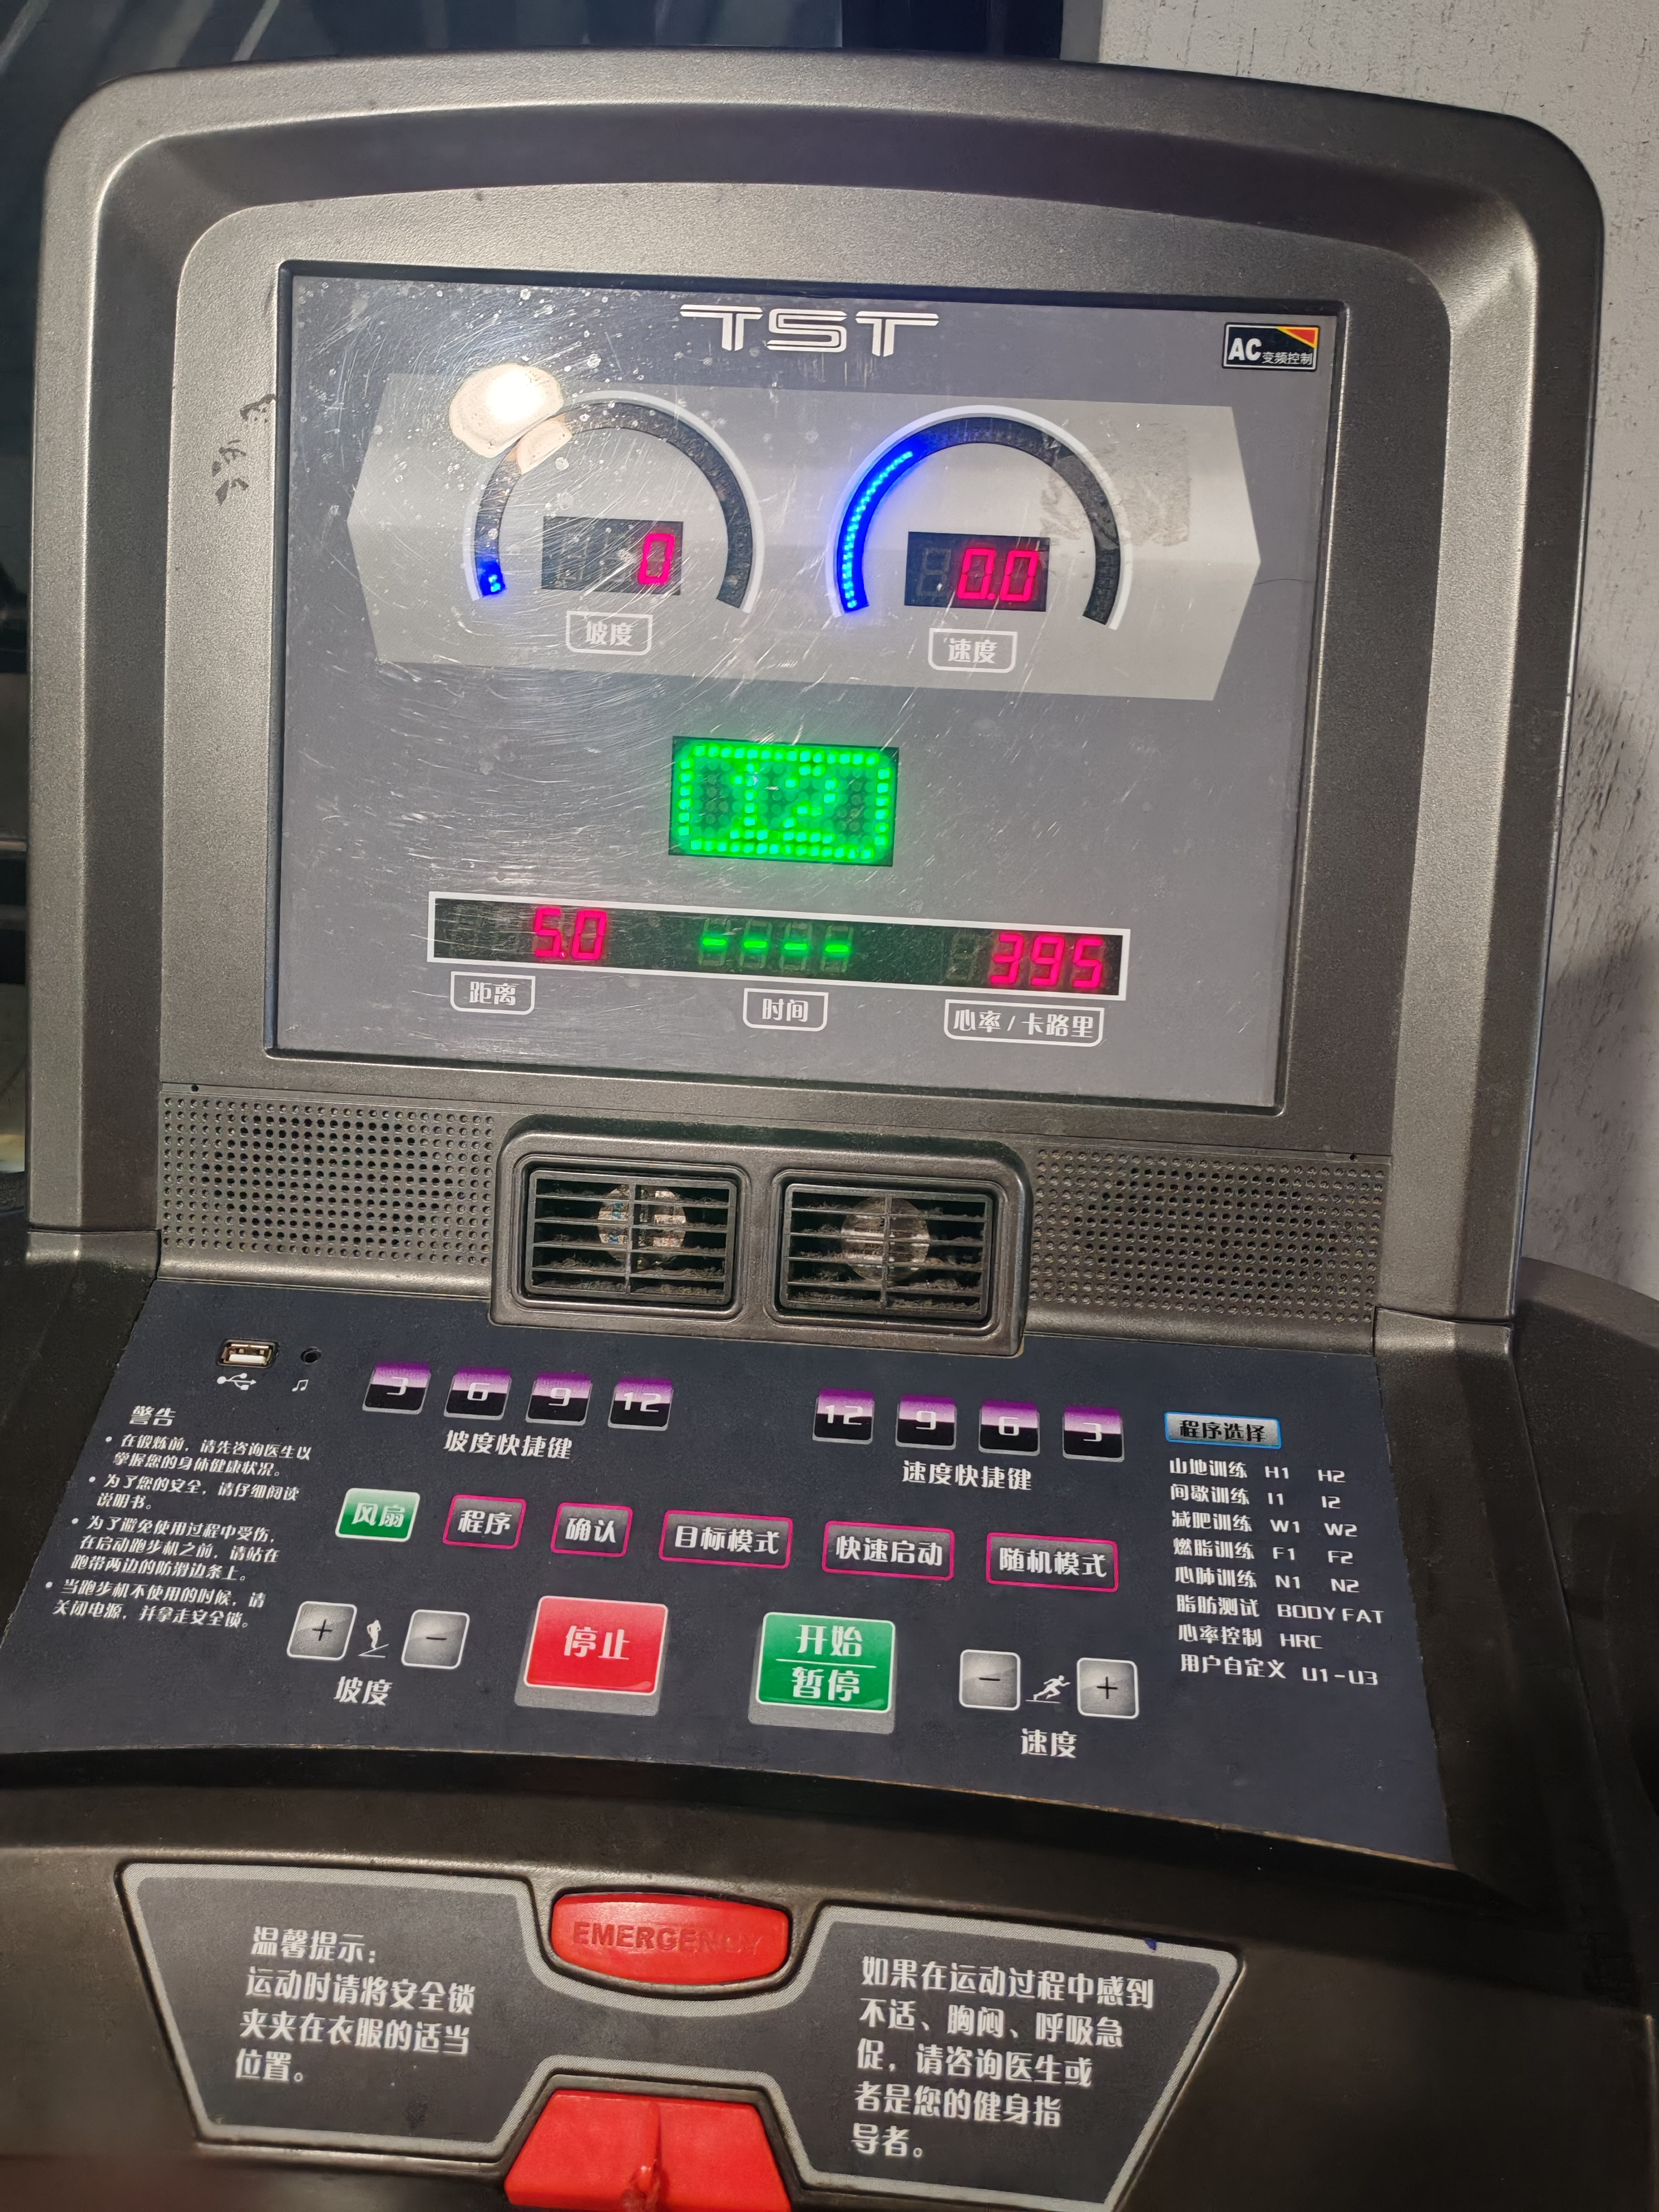
\includegraphics[width=0.72\columnwidth]{6.png}
        \caption{老师签字的原始数据}
    \end{figure}
\end{document}
